% !TeX root = ../../main.tex

\subsection{2-DOF Arm Gym Base Non-Distributed Experiment}

This experiment is the base experiment of a set of experiments for reinforcement learning in robots simulations.
In this way, we perform an initial experiment with a selected base reinforcement learning algorithm on 2-DOF robotics arm to achieve the goal of the environment and reach the target as quickly and efficiently as possible.
Based on this experiment, we plan to build on it more advanced experiments to show the effect of using distribution for reinforcement learning tasks and the benefit of parallelizing the environments to enhance the performance of the agents and solve the task quickly. Performing the experiment, we plan to extend it to a more complex environment with modified reward function and on different physics engine to compare between the existing reinforcement learning platforms and express the difference in comparison. Hence, we study the effect of distribution and transferability between different engine and the efficiency between them.

\subsubsection{Aim of the experiment}
% 1. Question behind (in the heading, why interesting, what to investigate)

This experiment is designed to be performed on non-distributed setup using only the power of CPUs, which make it the base experiment for our experiments and to be able to compare between different selected reinforcement learning methods and algorithms and show the effect of using distributed algorithms and parallelizing experiment's environment to achieve the efficiency and speed wanted to perform reinforcement learning experiments. 

We want to investigate how the agent will perform in the experiment, the time taken to run the experiment, the average episode reward the agent will get and whether the agent will be able to solve the environment in a constrained stopping conditions.

\subsubsection{Setup and configurations}

In this section we describe the setup of the experiment and how it was performed. Firstly, we introduce and describe the RoboReacher robotics arm environment provided by OpenAI Gym and PyBullet physics simulator. Then, based on the environment description, we present the observation space, action space and reward function of the experiment as a base towards the learning process and achieving environment goal. Subsequently, we describe the learning process. For this, we present the reinforcement learning algorithm and neural network architecture used.


\subsubsection{Environment Description: Roboschool Reacher}
Roboschool is an open-source software for robot simulation, integrated with OpenAI Gym. Our selected environment is \textit{Reacher Environment}~\ref{fig:openai_reacher}: A robotic arm consist of two linked joints places in a squared arena surrounding it along with a moving sphere (target). The goal of the robotics arm it to reach target sphere and maintain following the point until the end of the episode. 

\begin{figure}[!htb]
		\centering
				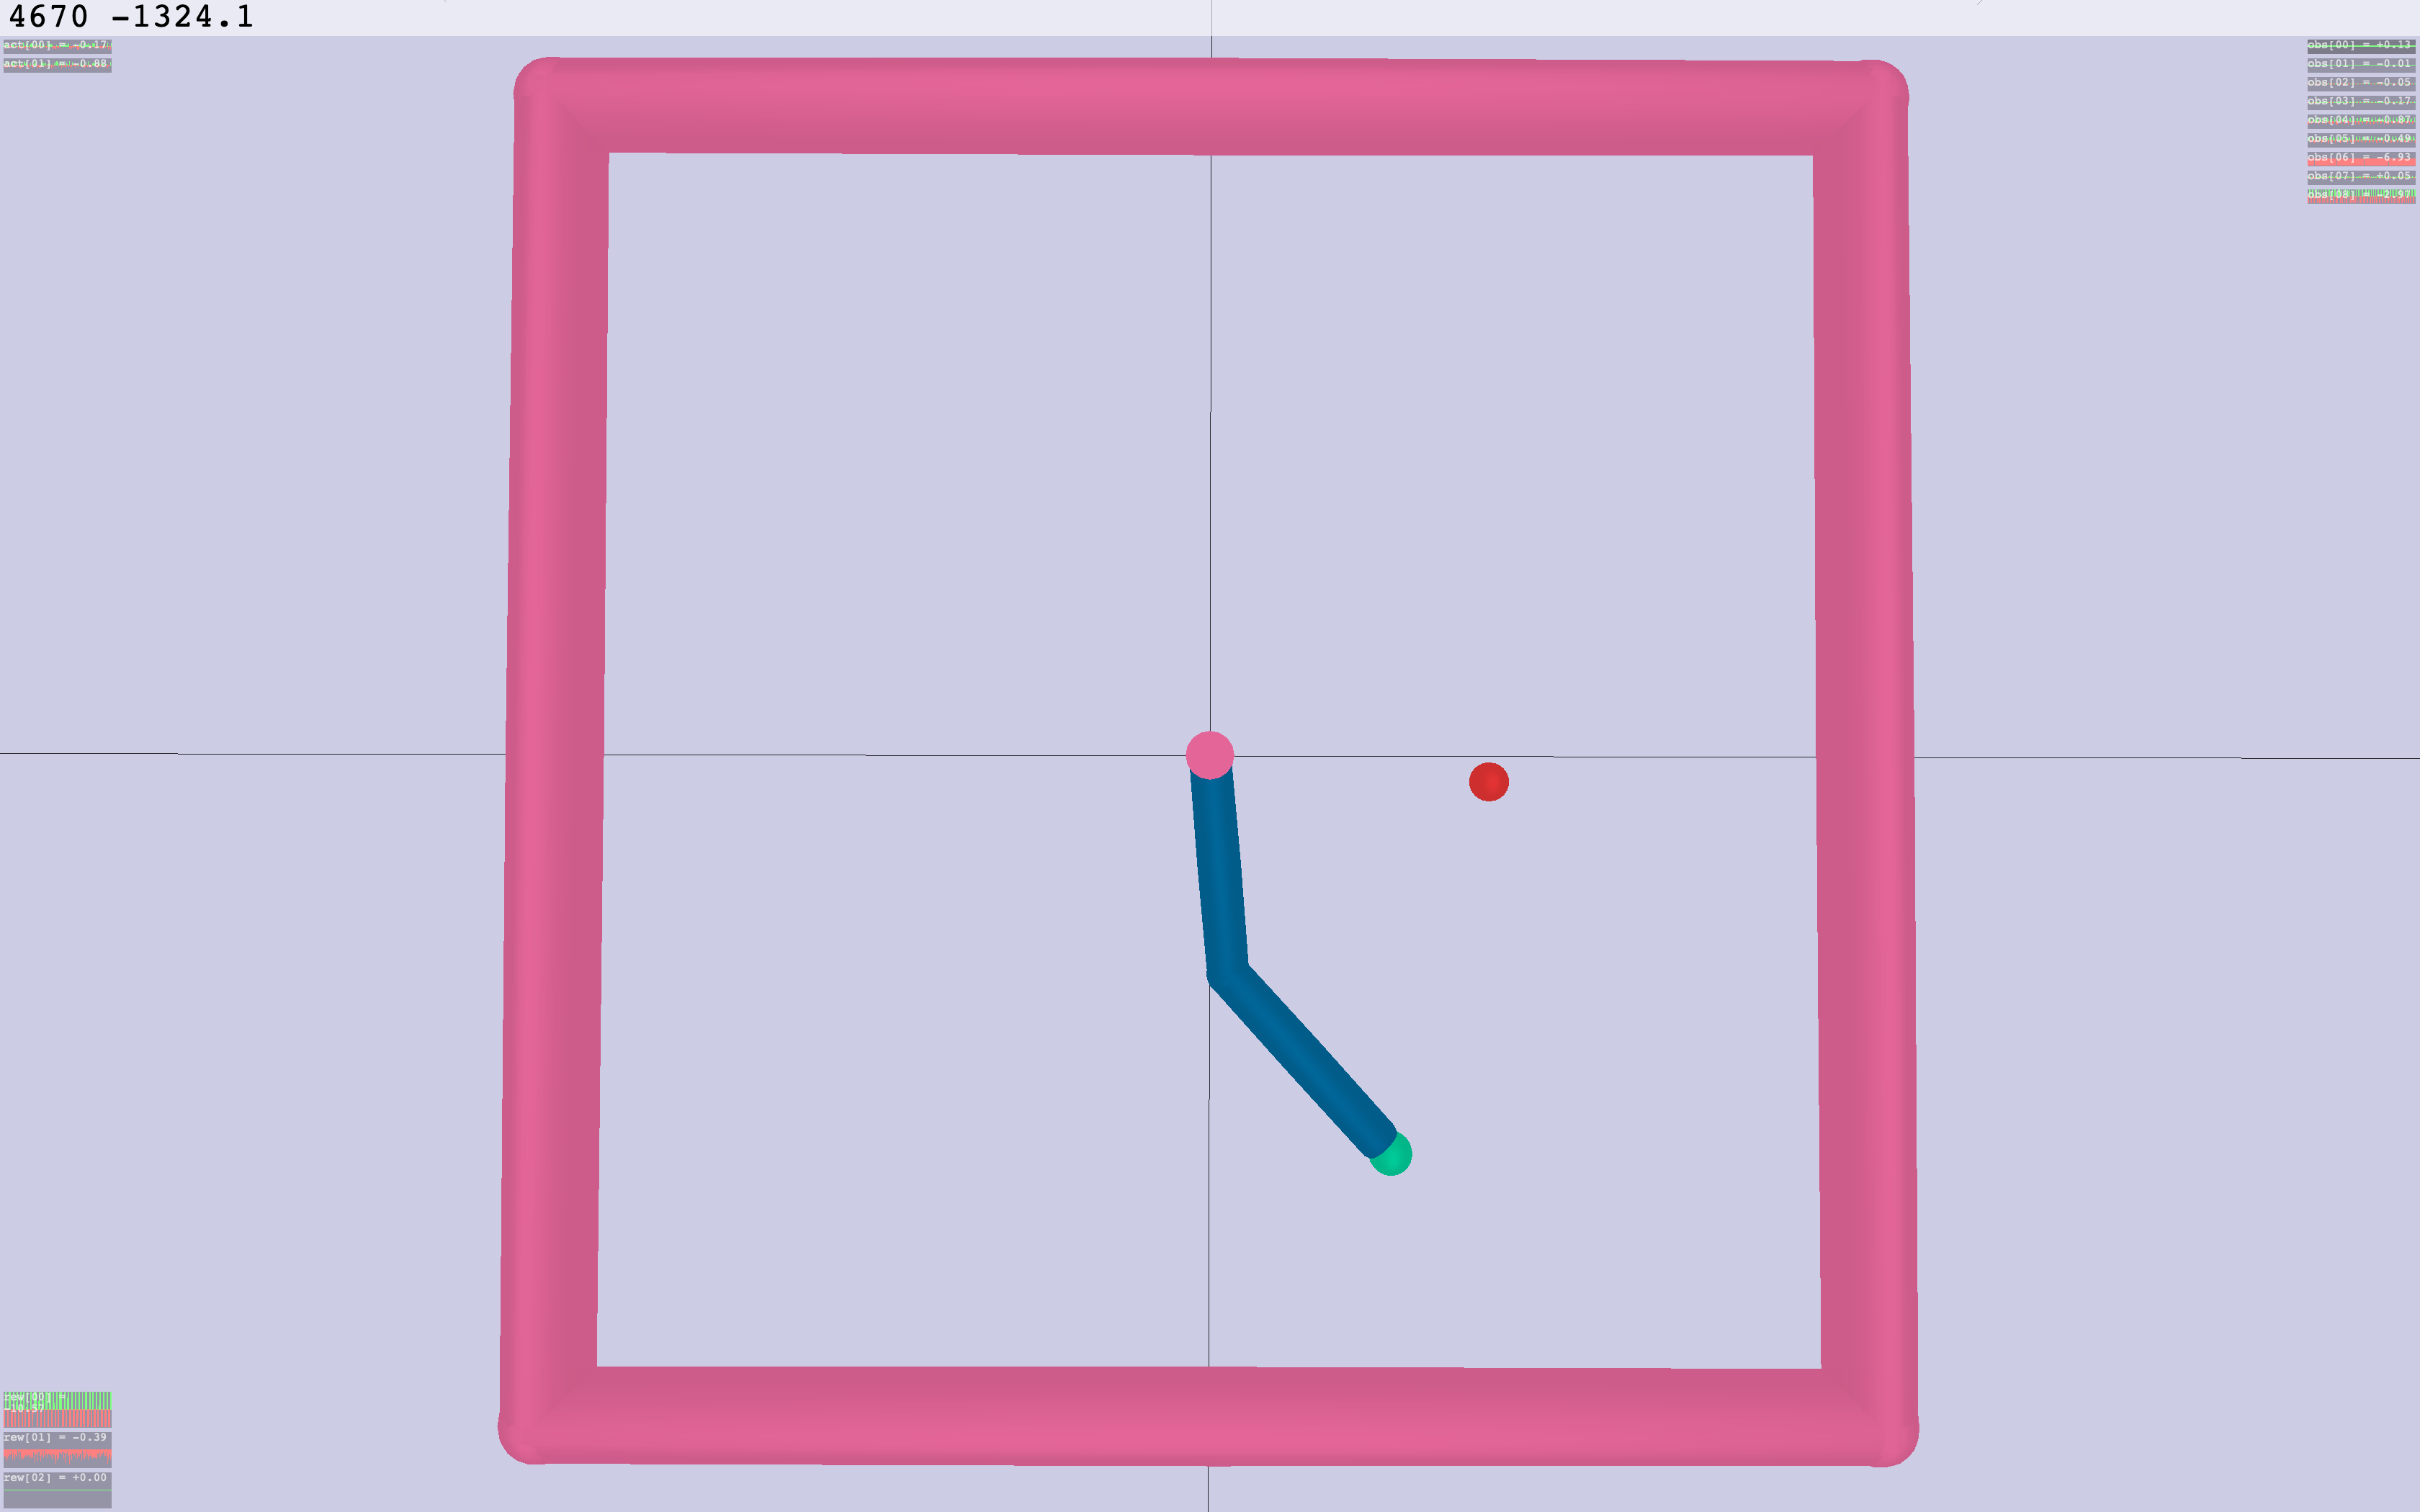
\includegraphics[width=0.7\linewidth]{figures/envs/openai_roboreacher.png}
				\caption{OpenAI Reacher Environment}
				\label{fig:openai_reacher}
\end{figure}

\subsubsection{Observation Space}

The observation space of the environment consist of 9 variables corresponding to the position of the target sphere, the x-axis and y-axis components of the vector from the target to the fingertip, cos(theta) and sin(theta) for the joints and the angular velocity of the fingertip in the x and y directions.

\begin{table}[!htb]
		\centering
		\begin{tabular}{|c|c|}
				\hline
				\multicolumn{2}{|c|}{{\ul \textit{\textbf{Observation Space}}}}                                                                                   \\ \hline
				\multirow{2}{*}{\textbf{Target Position}}                                                                      & \textit{X Position}              \\ \cline{2-2} 
																																																								& \textit{Y Position}              \\ \hline
				\multirow{2}{*}{\textbf{Arm to Target Vector}}                                                                 & \textit{Position vector 0}       \\ \cline{2-2} 
																																																								& \textit{Position vector 1}       \\ \hline
				\multirow{2}{*}{\textbf{\begin{tabular}[c]{@{}c@{}}Current Relative Position\\ of Central Joint\end{tabular}}} & \textit{cosine of central joint} \\ \cline{2-2} 
						& \textit{sine of central joint}   \\ \hline
				\multirow{2}{*}{\textbf{\begin{tabular}[c]{@{}c@{}}Current Relative Position\\ of Elbow Joint\end{tabular}}}   & \textit{cosine of elbow joint}   \\ \cline{2-2} 
						& \textit{sine of elbow joint}     \\ \hline
		\end{tabular}
		\caption{Gym Reacher Observation Information}
		\label{tab:gym_reacher_obs}
\end{table}

\subsubsection{Action Space}

The action space of the environment is a continuous one which indicated the torque applied on both of the robotic arm joints.


\begin{table}[!htb]
		\centering
		\begin{tabular}{|c|c|}
				\hline
				\multicolumn{2}{|c|}{{\ul \textit{\textbf{Action Space (Continuous)}}}}                             \\ \hline
				\multirow{2}{*}{\textbf{Center Joint Torque}} & \multirow{2}{*}{\textit{range(-1, 1)}} \\
																												&                                        \\ \hline
				\multirow{2}{*}{\textbf{Elbow Joint Torque}}  & \multirow{2}{*}{\textit{range(-1, 1)}} \\
																												&                                        \\ \hline
		\end{tabular}
				\caption{Gym Reacher Action Information}
				\label{tab:gym_reacher_actions}
\end{table}

\subsubsection{Reward Function}

The reward function is designed based on the distance between the arm and the target along with electricity cost of the torque and angular velocity of the arm with small epsilon amount in case of the joint is stuck. 

\subsubsection{Algorithm}

In this experiment, Proximal Policy Optimization (PPO) algorithm is selected to be the base algorithm for our initial experiment. PPO’s clipped objective supports multiple SGD passes over the same batch of experiences along with multi-GPU optimizer pins that data in GPU memory to avoid unnecessary transfers from host memory, substantially improving performance over a naive implementation. Since PPO scales out using multiple workers for experience collection, and also with multiple GPUs for SGD, it is preferable to compare it in using only CPU power in non distributed setup and when scaling the algorithm to have multiple worker and using multi-GPU optimization for faster training.

Below are the default configuration for PPO algorithm:
\lstinputlisting[language=Python]{chapters/04/ppo_default.py}

followed by this experiment setup and configuration as listed below:
\begin{table}[!htb]
		\centering
		\begin{tabular}{|c|l|l|c|l|l|}
				\hline
				\multicolumn{6}{|c|}{\textit{\textbf{Gym Reacher PPO 1st Experiment: Non-Distributed Experiment}}}                                                        \\ \hline
				\multicolumn{3}{|c|}{\textbf{env}}                                  & \multicolumn{3}{c|}{RoboschoolReacher-v1}                                           \\ \hline
				\multicolumn{3}{|c|}{\textbf{env\_type}}                            & \multicolumn{3}{c|}{OpenAI Environment}                                             \\ \hline
				\multicolumn{3}{|c|}{\textbf{run: Algorithms}}                      & \multicolumn{3}{c|}{\cellcolor[HTML]{C0C0C0}\textbf{PPO}}                           \\ \hline
				\multicolumn{3}{|c|}{}                                              & \multicolumn{3}{c|}{\cellcolor[HTML]{E1F7E1}episode\_reward\_mean = 21}             \\ \cline{4-6} 
				\multicolumn{3}{|c|}{\multirow{-2}{*}{\textbf{stop condition}}}     & \multicolumn{3}{c|}{\cellcolor[HTML]{E1F7E1}time-steps\_total = 10000000: 10M Steps} \\ \hline
				\multicolumn{3}{|c|}{\textbf{gamma}}                                & \multicolumn{3}{c|}{0.99}                                                           \\ \hline
				\multicolumn{3}{|c|}{\textbf{kl coefficient}}                            & \multicolumn{3}{c|}{1.0}                                                            \\ \hline
				\multicolumn{3}{|c|}{\textbf{num\_sgd\_iter}}                       & \multicolumn{3}{c|}{20}                                                             \\ \hline
				\multicolumn{3}{|c|}{\textbf{lr}}                                   & \multicolumn{3}{c|}{0.0001}                                                         \\ \hline
				\multicolumn{3}{|c|}{\textbf{sgd\_minibatch\_size}}                 & \multicolumn{3}{c|}{1000}                                                           \\ \hline
				\multicolumn{3}{|c|}{\textbf{train\_batch\_size}}                   & \multicolumn{3}{c|}{25000}                                                          \\ \hline
				\multicolumn{3}{|c|}{\textbf{batch\_mode}}                          & \multicolumn{3}{c|}{complete\_episodes}                                             \\ \hline
				\multicolumn{3}{|c|}{\textbf{observation\_filter}}                  & \multicolumn{3}{c|}{MeanStdFilter}                                                  \\ \hline
				\multicolumn{3}{|c|}{\cellcolor[HTML]{C0C0C0}\textbf{num\_gpus}}    & \multicolumn{3}{c|}{\cellcolor[HTML]{C0C0C0}0}                                      \\ \hline
				\multicolumn{3}{|c|}{\cellcolor[HTML]{C0C0C0}\textbf{num\_workers}} & \multicolumn{3}{c|}{\cellcolor[HTML]{C0C0C0}0}                                      \\ \hline
		\end{tabular}
		\caption{Gym Reacher PPO 1st Experiment: Non-Distributed Experiment}
		\label{tab:gym_reacher_ppo_1st_exp}
\end{table}


\subsubsection{Neural Network Architecture}
Since our observation space is not a visual observation, which means it won't require a convolutional neural network to process it, we will be using fully connected neural network consist of two hidden layers with 256 neuron for each layer as shown below~\ref{fig:ppo_nn}:

\begin{figure}[!htb]
		\centering
				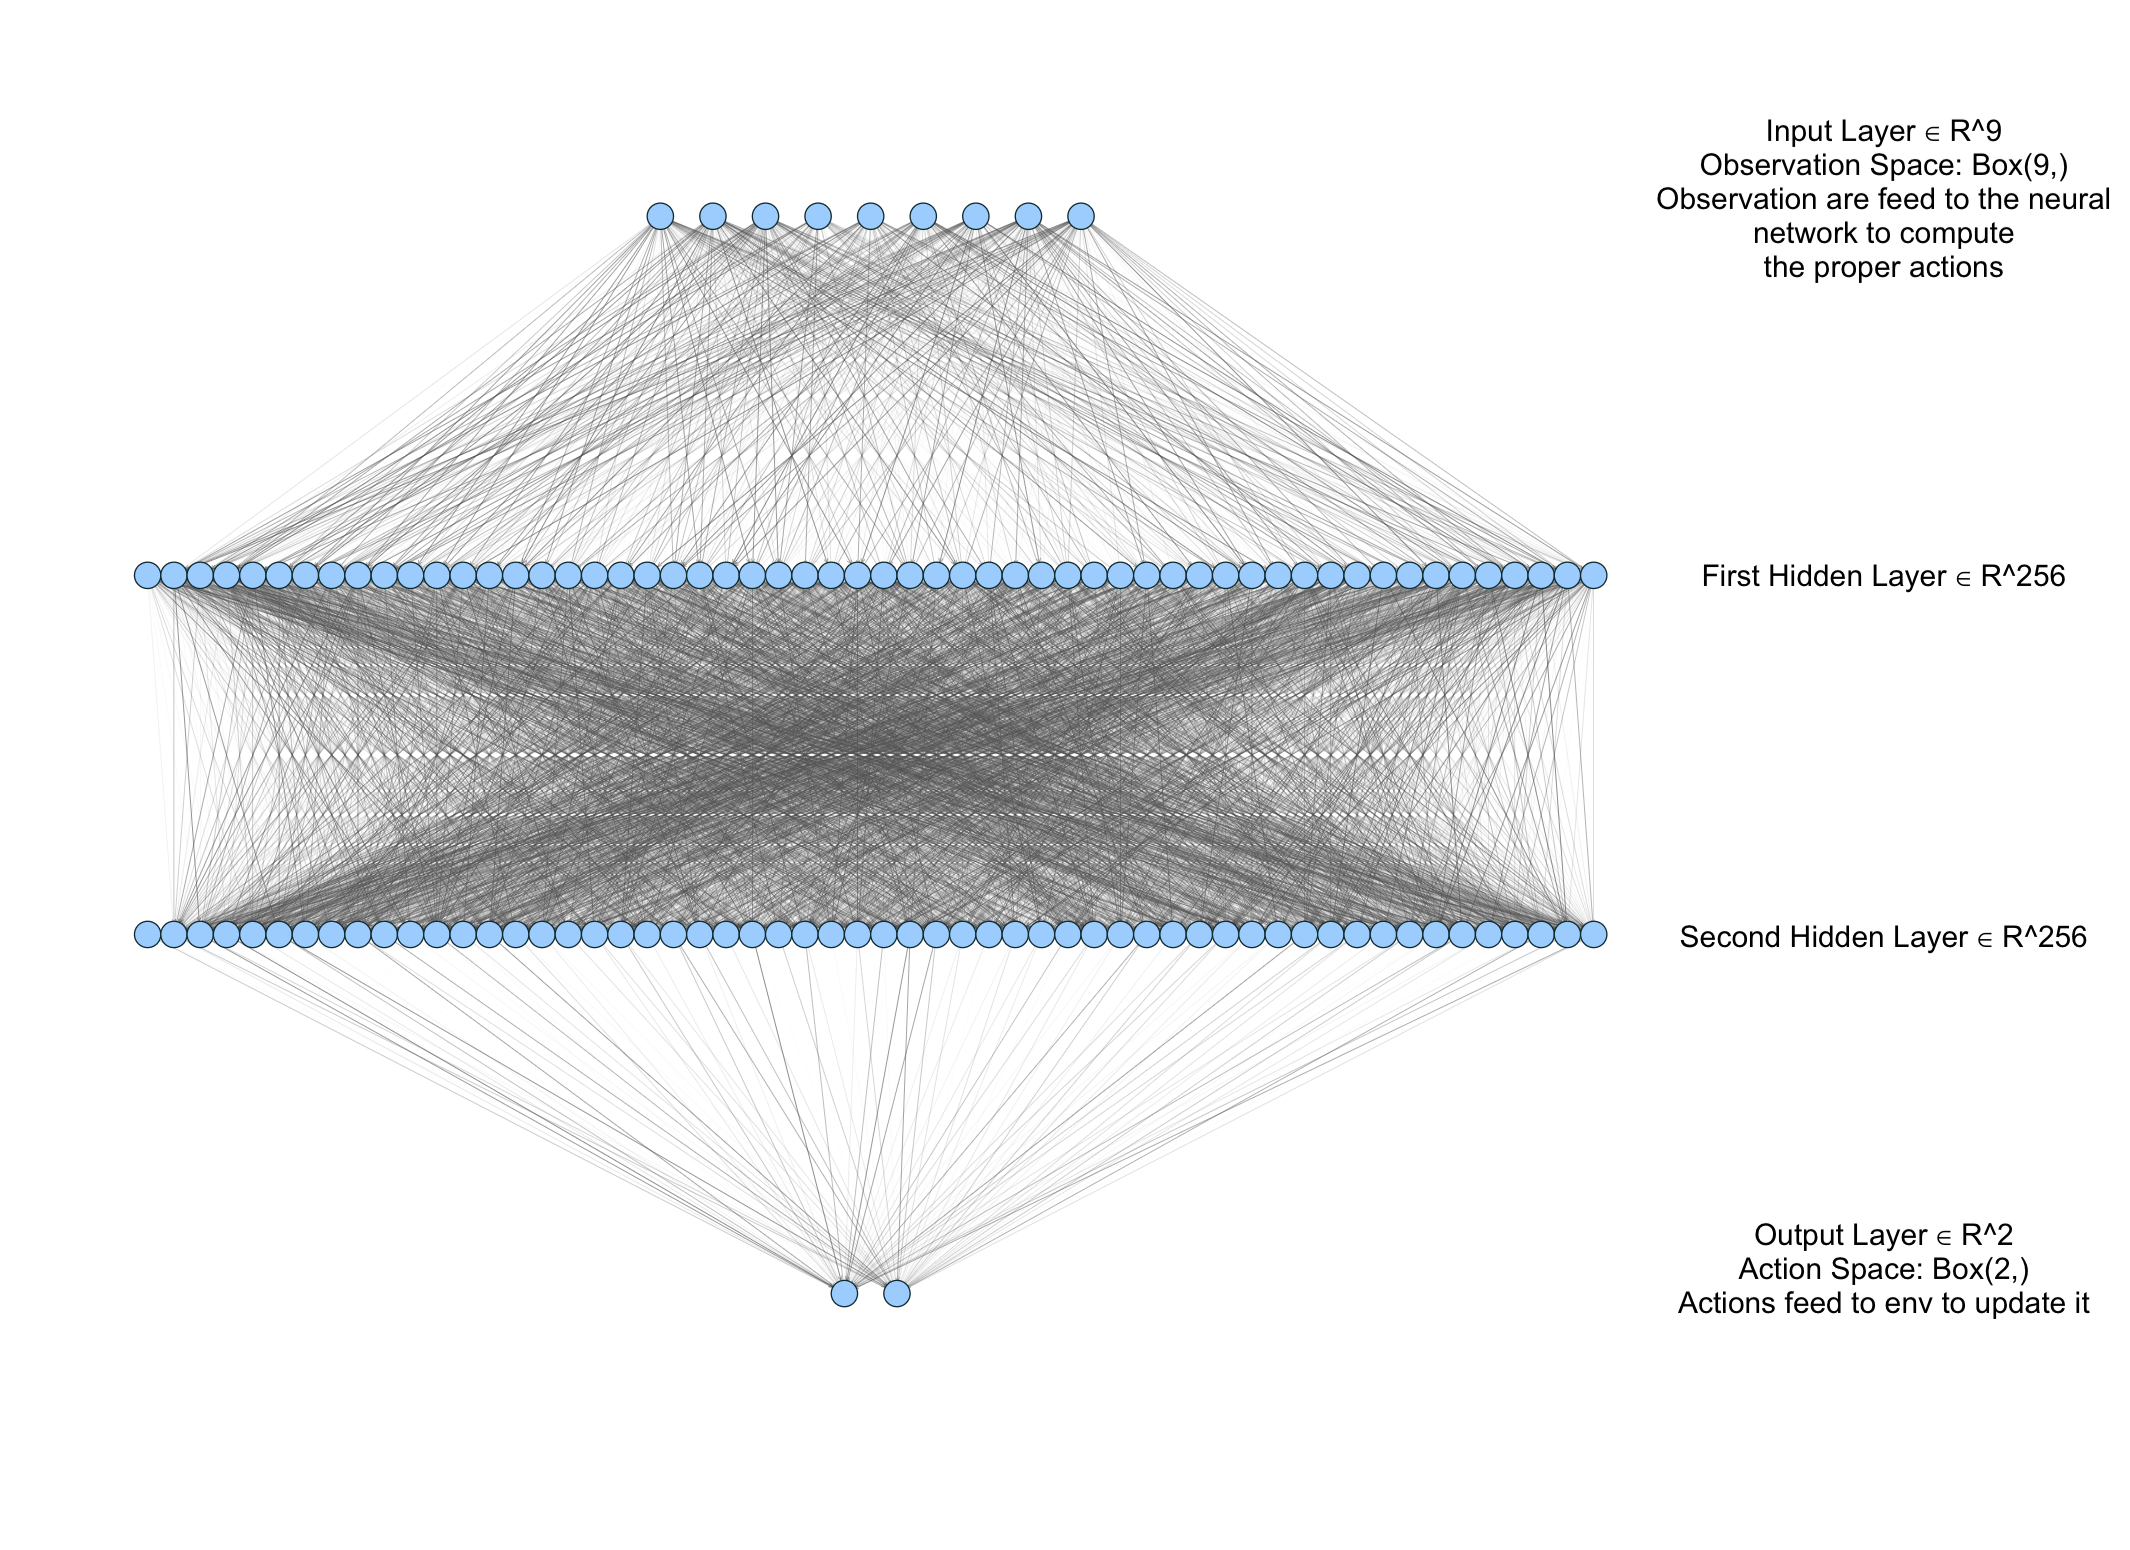
\includegraphics[width=\linewidth]{figures/exps/1st_exp/ppo_nn}
				\caption{PPO Neural Network Architecture}
				\label{fig:ppo_nn}
\end{figure}


\subsubsection{Experiment Results}

After running the experiment with a stopping conditions either reaching an average reward of 21 or total time steps of the agent is 10M steps as indicated in ~\ref{tab:gym_reacher_ppo_1st_exp}.
we observe that:

\begin{itemize}
		\item The agent completed the 10M steps.
		\item The agent could not solve the required task.
		\item The average the agent could get did not exceed 1 reward over the whole episodes~\ref{fig:avg_eps_reward}.
		\item The maximum the agent could get did not exceed 30 reward over the whole episodes~\ref{fig:max_eps_reward}.
		\item The performance of the agent is not quite good.
		\item The total loss (Policy~\ref{fig:policy_loss} + Value function~\ref{fig:vf_loss}) is not improving and didn't reach global minimum~\ref{fig:total_loss}.
		\item The total time elapsed exceed 3.5 hours for such a simple environment and task~\ref{fig:avg_reward_time}.
\end{itemize}

\begin{figure}[!htb]
		\centering
		\begin{subfigure}[!htb]{0.35\textwidth}
				\centering
				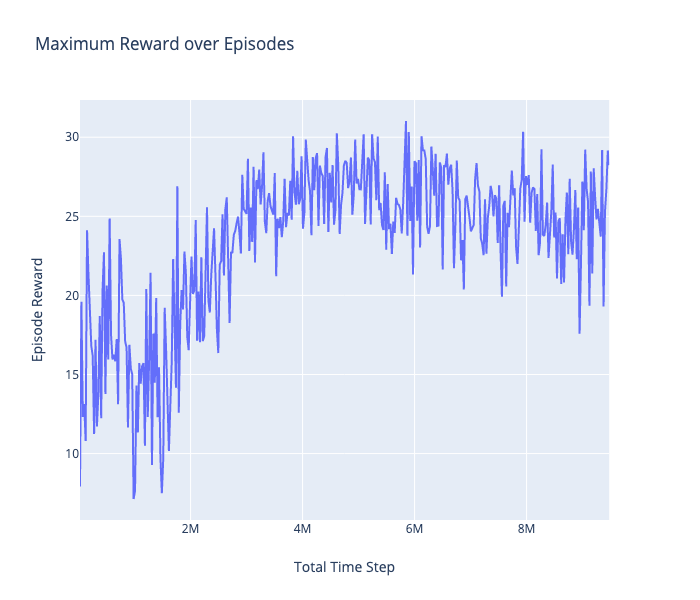
\includegraphics[width=\textwidth]{figures/exps/1st_exp/max_eps_reward}
				\caption{Maximum Reward over Episodes}
				\label{fig:max_eps_reward}
		\end{subfigure}
		\hfill
		\begin{subfigure}[!htb]{0.35\textwidth}
				\centering
				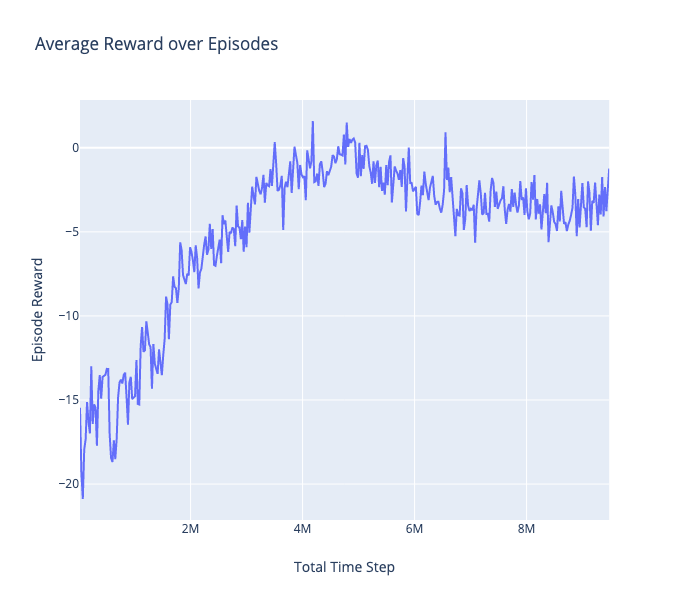
\includegraphics[width=\textwidth]{figures/exps/1st_exp/avg_eps_reward}
				\caption{Average Reward over Episodes}
				\label{fig:avg_eps_reward}
		\end{subfigure}
		\hfill

		\begin{subfigure}[!htb]{0.35\textwidth}
				\centering
				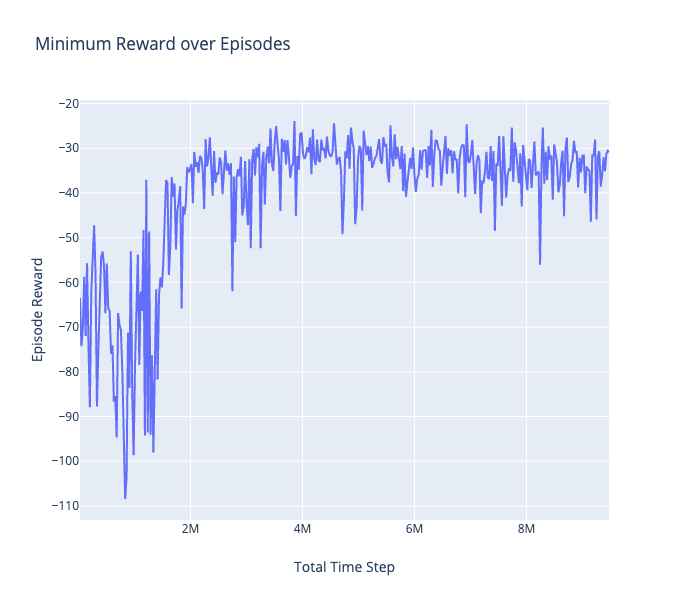
\includegraphics[width=\textwidth]{figures/exps/1st_exp/min_eps_reward}
				\caption{Minimum Reward over Episodes}
				\label{fig:min_eps_reward}
		\end{subfigure}
		\hfill
		\begin{subfigure}[!htb]{0.35\textwidth}
				\centering
				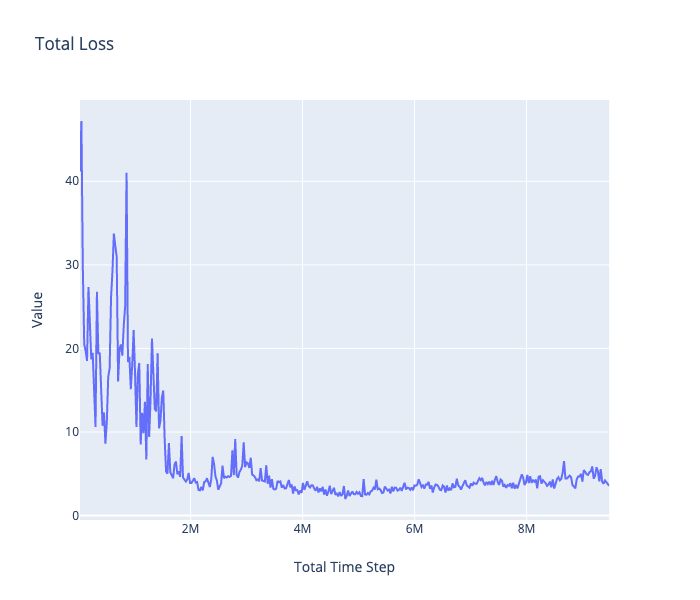
\includegraphics[width=\textwidth]{figures/exps/1st_exp/total_loss}
				\caption{Total Loss}
				\label{fig:total_loss}
		\end{subfigure}
		\hfill

		\begin{subfigure}[!htb]{0.35\textwidth}
				\centering
				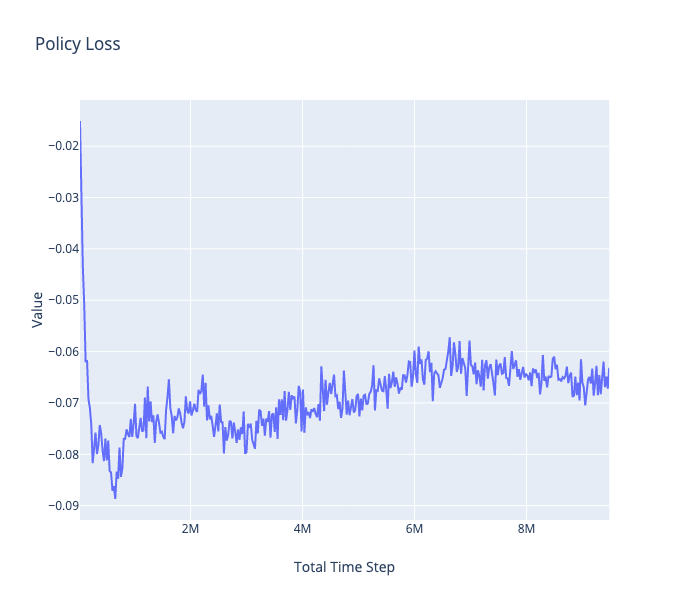
\includegraphics[width=\textwidth]{figures/exps/1st_exp/policy_loss}
				\caption{Policy Loss}
				\label{fig:policy_loss}
		\end{subfigure}
		\hfill
		\begin{subfigure}[!htb]{0.35\textwidth}
				\centering
				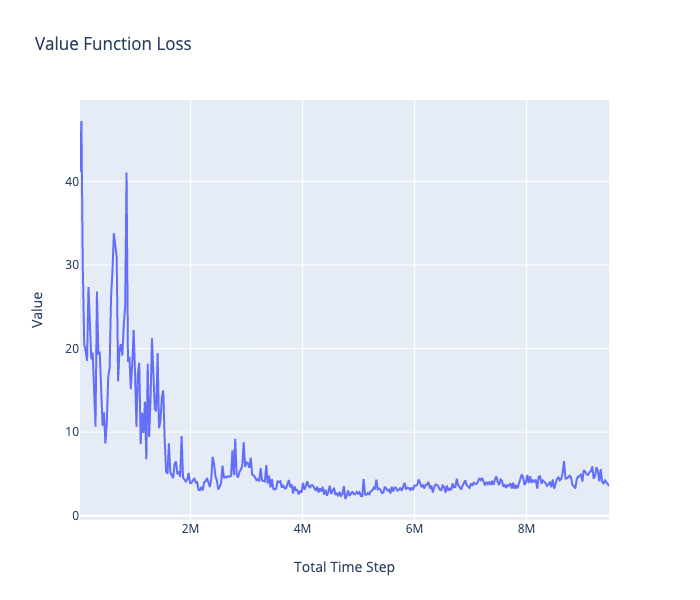
\includegraphics[width=\textwidth]{figures/exps/1st_exp/vf_loss}
				\caption{Value Function Loss}
				\label{fig:vf_loss}
		\end{subfigure}
		\hfill

		\begin{subfigure}[!htb]{0.35\textwidth}
				\centering
				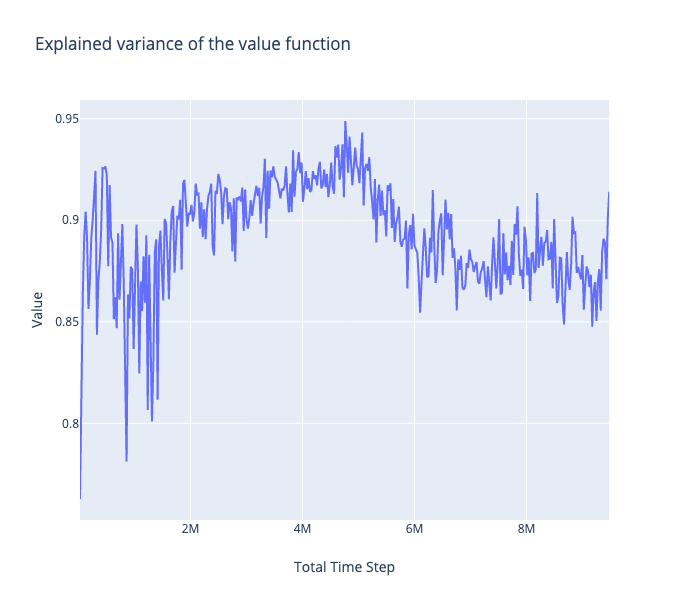
\includegraphics[width=\textwidth]{figures/exps/1st_exp/vf_explained_var}
				\caption{Explained variance of the value function}
				\label{fig:vf_explained_var}
		\end{subfigure}
		\hfill
		\begin{subfigure}[!htb]{0.35\textwidth}
				\centering
				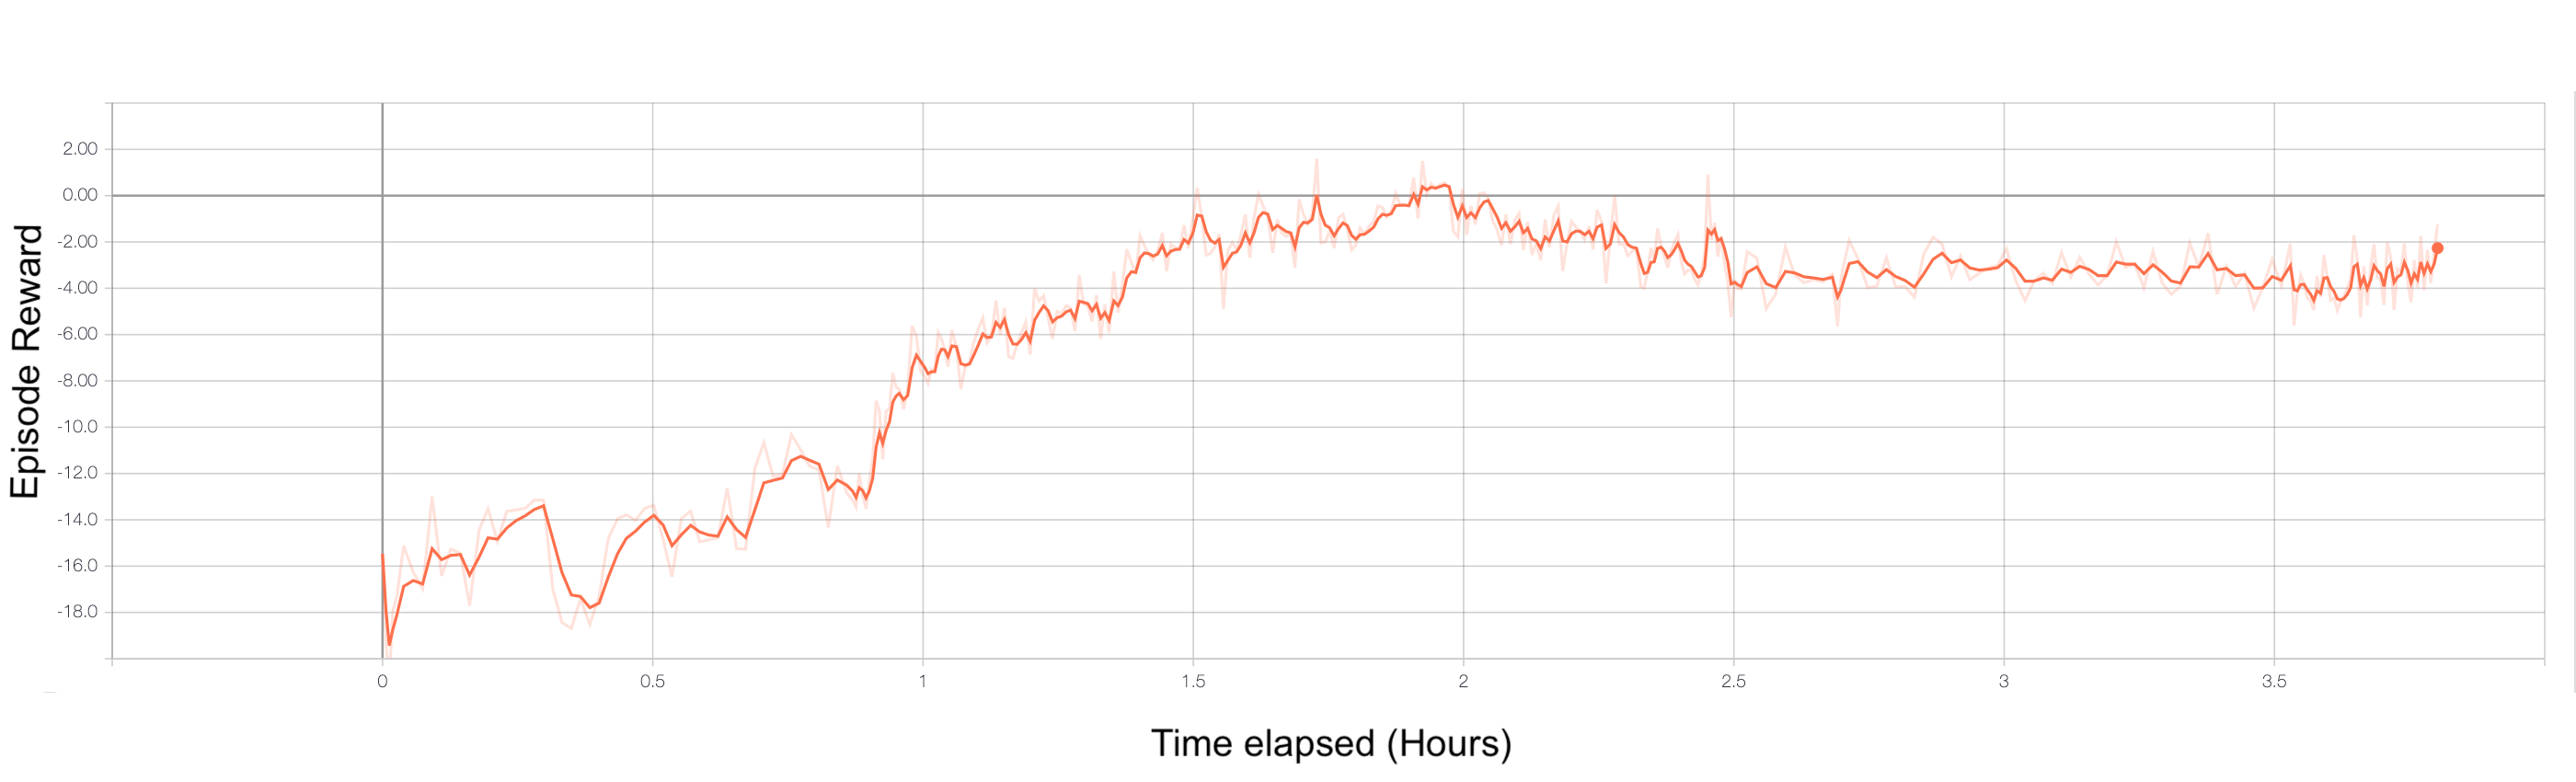
\includegraphics[width=\textwidth]{figures/exps/1st_exp/avg_reward_time}
				\caption{Average Reward over Episodes | Time Elapsed}
				\label{fig:avg_reward_time}
		\end{subfigure}
		\hfill

		 \caption{RoboReacher Gym Base Environment: Non-Distributed Experiment Results}
		 \label{fig:1st_exp_results}
\end{figure}

\subsubsection{Conclusion}

In this experiment, we perform a training and evaluation for the simple robotic task using ppo algorithm in non-distributed setup to train our agent. we conclude that the experiment took a large amount of time to train the agent (4 hours) and at the end the agent didn't solve the required task and the learning process was not successful. 